\begin{figure}[H]
	\centering
	\subfloat[][DCAP\_3\_3\_3\_3]
	{
		\centering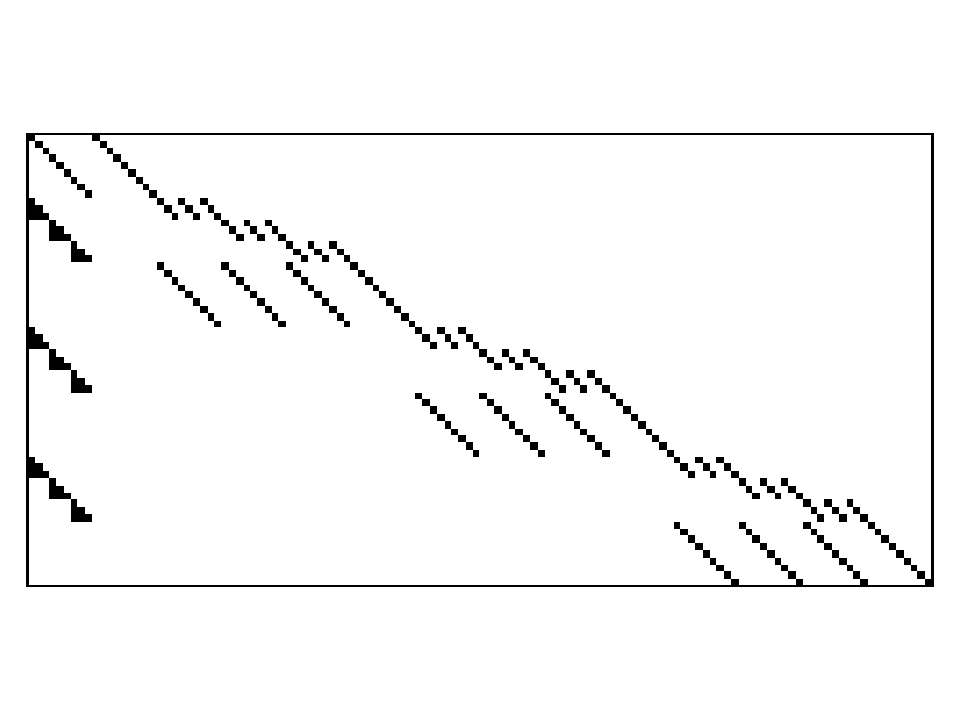
\includegraphics[width=0.45\linewidth]{DCAP_3_3_3_3}
		\label{fig:de_structure_dcap}
	}
	~
	\subfloat[][MPTSPs\_D0\_3\_3]
	{
		\centering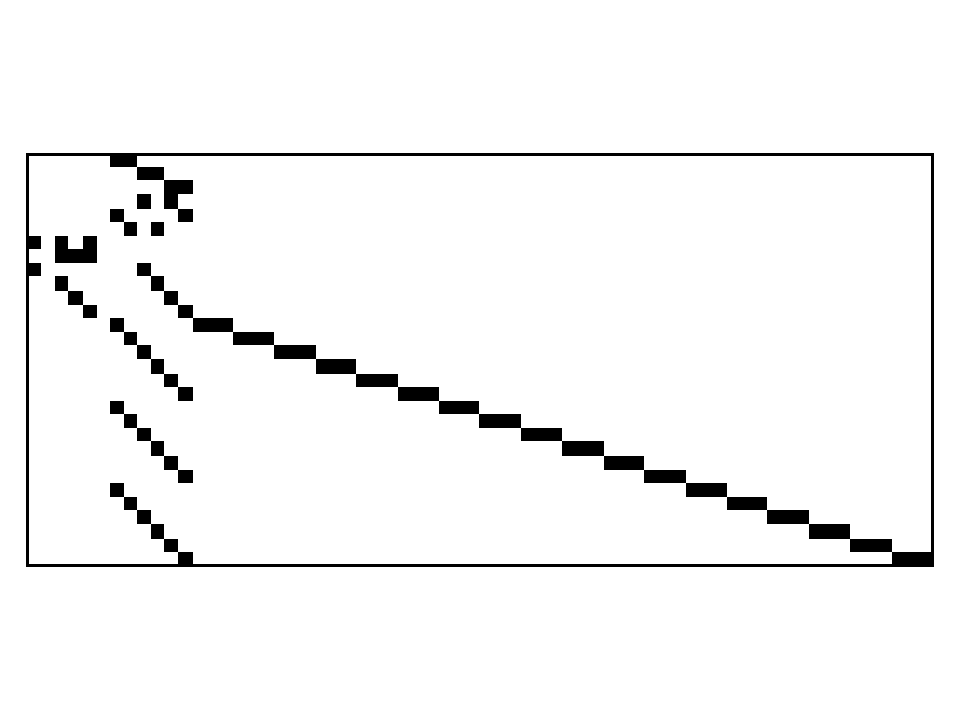
\includegraphics[width=0.45\linewidth]{MPTSPs_D0_3_3}
		\label{fig:de_structure_mptsps}
	}
	
	\subfloat[][SIZES\_3]
	{
		\centering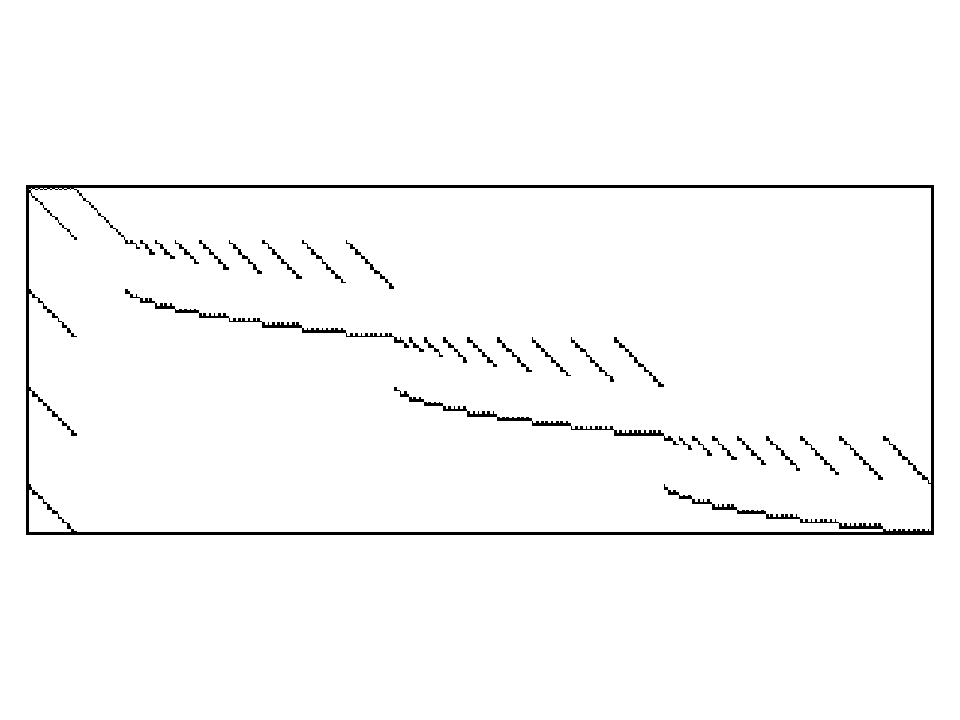
\includegraphics[width=0.45\linewidth]{SIZES_3}
		\label{fig:de_structure_sizes}
	}
	~
	\subfloat[][SMKP\_120\_3]
	{
		\centering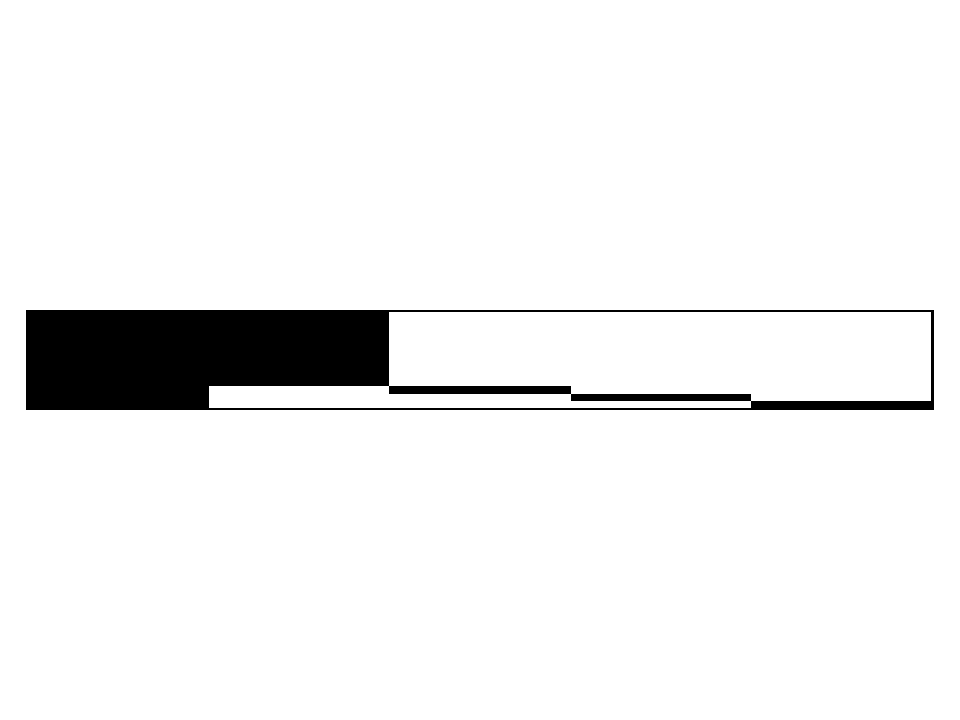
\includegraphics[width=0.45\linewidth]{SMKP_120_3}
		\label{fig:de_structure_smkp}
	}
	
	\subfloat[][SSLP\_5\_10\_3]
	{
		\centering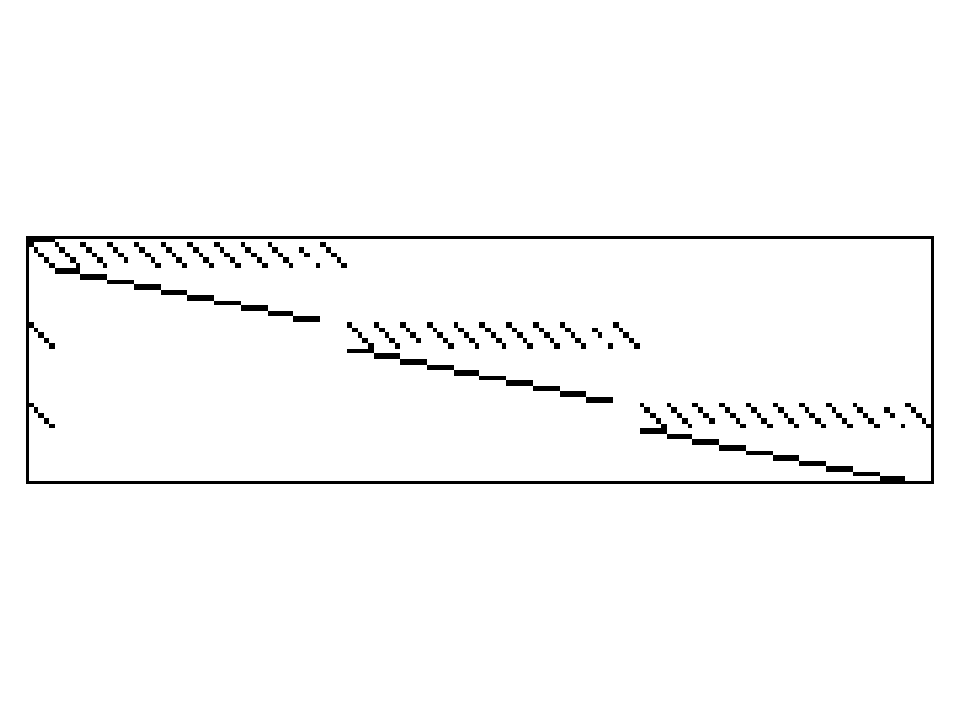
\includegraphics[width=0.45\linewidth]{SSLP_5_10_3}
		\label{fig:de_structure_sslp}
	}
	~
	\subfloat[][SUC\_FallWD\_1]
	{
		\centering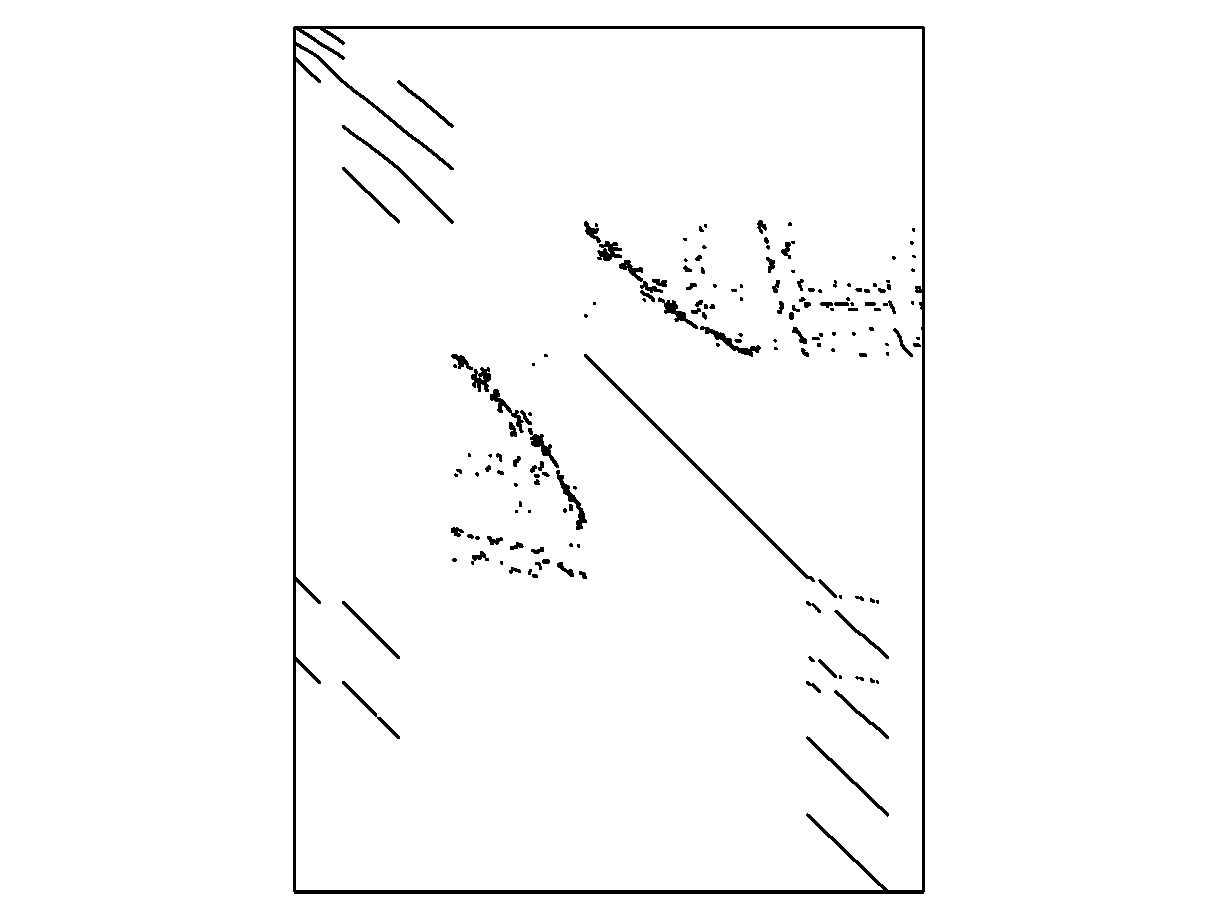
\includegraphics[width=0.45\linewidth]{SUC_FallWD_1}
		\label{fig:de_structure_sucw}
	}

	\caption{Block-diagonal structure in extensive form}
%	\begin{minipage}
%		{0.65\textwidth}{\footnotesize *\suc\ instance is too huge and extremely sparse to plot more than 1 scenario}
%	\end{minipage}
	\label{fig:de_structure}
\end{figure}